\documentclass[11pt,a4paper]{article}

% ─── Core Packages ───────────────────────────────────────────────────────────
\usepackage[margin=1in]{geometry}
\usepackage[T1]{fontenc}
\usepackage{lmodern}
\usepackage{amsmath,amssymb,amsthm}
\usepackage{mathtools}
\usepackage{graphicx}
\usepackage{xcolor}
\usepackage{booktabs}
\usepackage{multirow}
\usepackage{array}
\usepackage{enumitem}
\usepackage{algorithm}
\usepackage{algpseudocode}
\usepackage{tcolorbox}
\usepackage{microtype}
\usepackage{caption}
\usepackage{natbib}
\usepackage{tikz}
\usepackage{pgfplots}
\pgfplotsset{compat=1.18}
\usetikzlibrary{positioning,arrows.meta,shapes.geometric,fit}
\usepackage{listings}
\usepackage{hyperref}
\usepackage[noabbrev]{cleveref}

% ─── Color Definitions ───────────────────────────────────────────────────────
\definecolor{defbg}{RGB}{245,240,255}
\definecolor{defborder}{RGB}{130,70,200}
\definecolor{warnbg}{RGB}{255,245,235}
\definecolor{warnborder}{RGB}{200,130,70}
\definecolor{notebg}{RGB}{235,245,255}
\definecolor{noteborder}{RGB}{70,130,200}
\definecolor{codegray}{RGB}{245,245,245}
\definecolor{codekey}{RGB}{0,0,180}
\definecolor{codecomment}{RGB}{100,100,100}
\definecolor{codestring}{RGB}{160,32,32}

% ─── Listings Setup ──────────────────────────────────────────────────────────
\lstset{
  language=Python,
  basicstyle=\ttfamily\small,
  keywordstyle=\color{codekey}\bfseries,
  commentstyle=\color{codecomment}\itshape,
  stringstyle=\color{codestring},
  backgroundcolor=\color{codegray},
  frame=single, framerule=0.4pt, rulecolor=\color{gray!40},
  numbers=left, numberstyle=\tiny\color{gray}, numbersep=6pt,
  breaklines=true, showstringspaces=false, tabsize=2,
  xleftmargin=12pt, xrightmargin=4pt,
}

% ─── tcolorbox Environments ──────────────────────────────────────────────────
\tcbuselibrary{skins,breakable}

\newtcolorbox{definitionbox}[1][]{
  enhanced, breakable,
  colback=defbg, colframe=defborder,
  fonttitle=\bfseries\small,
  left=6pt, right=6pt, top=4pt, bottom=4pt,
  arc=4pt, #1}

\newtcolorbox{warnbox}[1][]{
  enhanced, breakable,
  colback=warnbg, colframe=warnborder,
  fonttitle=\bfseries\small, title={Failure Mode},
  left=6pt, right=6pt, top=4pt, bottom=4pt,
  arc=4pt, #1}

\newtcolorbox{notebox}[1][]{
  enhanced, breakable,
  colback=notebg, colframe=noteborder,
  fonttitle=\bfseries\small,
  left=6pt, right=6pt, top=4pt, bottom=4pt,
  arc=4pt, #1}

% ─── Math Operators ──────────────────────────────────────────────────────────
\DeclareMathOperator*{\argmin}{arg\,min}
\DeclareMathOperator*{\argmax}{arg\,max}
\DeclareMathOperator{\Softmax}{Softmax}
\DeclareMathOperator{\TopK}{Top\text{-}k}
\DeclareMathOperator{\Concat}{Concat}
\DeclareMathOperator{\Upsample}{Upsample}
\DeclareMathOperator{\reshape}{reshape}
\DeclareMathOperator{\flatten}{flatten}
\DeclareMathOperator{\IoU}{IoU}
\DeclareMathOperator{\simop}{sim}
\newcommand{\sg}[1]{\mathrm{sg}\!\left[#1\right]}

% ─── Math Shorthands ─────────────────────────────────────────────────────────
\newcommand{\R}{\mathbb{R}}
\newcommand{\E}{\mathbb{E}}
\newcommand{\vc}{\mathbf{v}_c}
\newcommand{\qe}{\mathbf{q}_e}
\newcommand{\vm}{\mathbf{m}}
\newcommand{\vs}{\mathbf{s}}
\newcommand{\mI}{\mathbf{I}}
\newcommand{\mQ}{\mathbf{Q}}
\newcommand{\mV}{\mathbf{V}}

% ─── Theorem Environments ────────────────────────────────────────────────────
\newtheorem{hypothesis}{Hypothesis}
\newtheorem{remark}{Remark}
\newtheorem{definition}{Definition}

% ─── Hyperref Setup ──────────────────────────────────────────────────────────
\hypersetup{
  colorlinks=true,
  linkcolor=defborder,
  citecolor=teal,
  urlcolor=noteborder,
  pdftitle={TC-ViTok: Task-Conditioned Visual Tokenization},
  pdfauthor={Muhammad Ali Shah and Talha Hassan Ul Haq}
}

% ════════════════════════════════════════════════════════════════════════════
\begin{document}
% ════════════════════════════════════════════════════════════════════════════

\title{
  \textbf{TC-ViTok: Task-Conditioned Visual Tokenizer} \\[0.3em]
  \large A Learned Token-Selection Policy for Efficient Vision-Language Reasoning
}

\author{
  Muhammad Ali Shah - Talha Hassan Ul Haq \\[0.3em]
  Lahore University of Management Sciences (LUMS) \\
  \texttt{\{27100172, 27100306\}@lums.edu.pk}
}

\date{\today}

\maketitle
\thispagestyle{empty}

% ────────────────────────────────────────────────────────────────────────────
\begin{abstract}
% ────────────────────────────────────────────────────────────────────────────

Vision-language models (VLMs) such as LLaVA encode every image into a
\emph{fixed} set of $N$ visual tokens regardless of the spatial specificity
of the language query.
This is fundamentally wasteful: a question like ``What is written on the
sign?''\ requires high-resolution attention to one small region, whereas ``Is
there a cat?''\ requires only coarse global features.
We introduce \textbf{TC-ViTok} (\textbf{T}ask-\textbf{C}onditioned
\textbf{Vi}sual \textbf{Tok}enizer), a lightweight module that \emph{learns
a token-selection policy}
$\pi_\theta\colon (\qe, \vc) \to \mathcal{S} \subseteq \{1,\ldots,N\}$,
mapping a CLIP language embedding and a coarse DINOv2 spatial feature map to a
sparse subset of $k \ll N$ visual tokens.
The core component is a \emph{Tokenization Policy Network} (TPN): a
cross-attention module that scores every spatial position by its
relevance to the query, trained end-to-end via a Gumbel-Sigmoid
straight-through estimator with a phased curriculum and compression
regularization.
Selected tokens are extracted via an index-gather operation, so the LLM
receives a sequence of length $k + L$ rather than $N + L$, reducing
LLM prefill attention cost by up to $75\%$ at $k{=}144$ ($4\times$
compression from $N{=}576$).
Unlike existing visual-token compression methods---all of which are
query-agnostic---TC-ViTok conditions the tokenization decision on the user's
natural-language query \emph{before} the selected tokens enter the language
model.
We evaluate on VQAv2, GQA, and TextVQA, and hypothesize that
query-conditioning yields selective improvements concentrated in
spatially-grounded questions---the precise regime where fixed-budget
tokenization is most harmful.

\end{abstract}

\tableofcontents
\newpage

% ════════════════════════════════════════════════════════════════════════════
\section{Introduction}
\label{sec:intro}
% ════════════════════════════════════════════════════════════════════════════

\subsection{The Fixed-Budget Problem}

Modern VLMs encode images into a fixed-length sequence of $N$ visual tokens,
each corresponding to one patch of the input.
LLaVA-1.5~\citep{liu2024llava} produces $N{=}576$ tokens from a
$336{\times}336$ image with a $14{\times}14$ patch size.
These tokens are concatenated with $L$ text tokens and fed to a causal
language model (LLM) whose self-attention cost is dominated by the
$\mathcal{O}(N(N{+}L))$ term arising from visual-token self-attention and
text-to-visual cross-attention.\footnote{
  In prefix-style VLMs, visual tokens serve as a prefix to which every
  subsequent text token attends.
  For a typical query length $L \approx 30$ and $N{=}576$, visual tokens
  contribute $\sim\!95\%$ of the total prefill attention cost.
}
Every query---whether it demands fine-grained spatial reading or coarse
scene-level understanding---receives the same 576-token budget.
The number of visual tokens is determined by image resolution, not by task
complexity.

\subsection{Limitations of Existing Compression Methods}

Several methods attempt to reduce the visual token count:
\begin{itemize}[leftmargin=1.5em, itemsep=2pt]
  \item \textbf{Token Merging (ToMe)}~\citep{bolya2022token}: merges
    visually similar tokens inside the ViT using bipartite soft matching.
    The criterion is embedding-space similarity---purely image-driven and
    query-agnostic.
  \item \textbf{LLaVA-PruMerge}~\citep{shang2024llava}: prunes tokens by
    their cross-attention weight with the \texttt{[CLS]} token, which
    summarizes the \emph{entire image} rather than the query.
    The full ViT forward pass still runs; savings accrue only in the LLM.
  \item \textbf{DynamicViT}~\citep{rao2021dynamicvit}: learns to drop
    tokens inside the ViT.
    Content-adaptive but not conditioned on any external task signal.
\end{itemize}
The shared limitation is that \textbf{the compression decision is made
without knowledge of the task}.
These methods learn which tokens are \emph{generally} important, not which
tokens are important \emph{for a specific question}.

\subsection{Our Approach: Tokenization as a Learned Policy}

We propose a conceptual shift: \textbf{visual tokenization should be a
learned, query-conditioned policy}.
A policy maps a state (the query--image pair) to an action (the selected
token set):
\begin{equation}
  \pi_\theta\colon (\qe,\, \vc) \;\longrightarrow\;
    \mathcal{S} \;\subseteq\; \{1, \ldots, N\},
    \qquad |\mathcal{S}| = k,
  \label{eq:policy_def}
\end{equation}
where $\qe \in \R^{d_q}$ is a CLIP text embedding of the query,
$\vc \in \R^{M \times d_c}$ is a coarse DINOv2 spatial feature map with
$M \ll N$ tokens, and $\theta$ are the learnable TPN parameters.
The selected tokens are extracted via an index-gather operation, producing
a compact visual sequence of length $k$ that is passed to the LLM.
This is distinct from zero-masking approaches that retain the full sequence
length but zero out unselected rows: gather reduces both FLOPs and memory in
the LLM prefill stage.

This framing makes a testable prediction: query-conditioning should help
\emph{selectively}, concentrated on spatially-grounded questions where
different queries require attention to different image regions.
For globally-answerable questions (e.g., scene classification), the benefit
should be negligible.

\subsection{Contributions}

\begin{enumerate}[leftmargin=1.5em, itemsep=2pt]
  \item \textbf{Formulation.}
    We formalize visual tokenization as a query-conditioned discrete policy
    and distinguish it from prior query-agnostic compression.
  \item \textbf{Architecture.}
    We introduce the \emph{Tokenization Policy Network} (TPN), a lightweight
    cross-attention module that produces spatial token-selection scores
    conditioned on the user's language query.
  \item \textbf{Efficient gather-based injection.}
    Selected tokens are extracted via \texttt{torch.gather} before the LLM,
    reducing LLM input sequence length from $N{+}L$ to $k{+}L$ and cutting
    prefill FLOPs by up to $75\%$ at $k{=}144$.
  \item \textbf{Training.}
    We propose a phased curriculum with Gumbel-Sigmoid annealing and
    compression regularization to train the discrete policy end-to-end.
  \item \textbf{Evaluation protocol.}
    We introduce a \emph{spatial specificity stratification} of VQA
    benchmarks, enabling fine-grained hypothesis testing of when
    query-conditioning helps.
\end{enumerate}

% ════════════════════════════════════════════════════════════════════════════
\section{Related Work}
\label{sec:related}
% ════════════════════════════════════════════════════════════════════════════

\paragraph{Vision-language architectures.}
Modern VLMs follow a recipe of visual encoder, projection layer, and LLM
backbone~\citep{liu2024llava,li2023blip2,bai2023qwenvl}.
LLaVA-1.5~\citep{liu2024llava} uses a CLIP ViT-L/14 encoder, a two-layer MLP
projector, and Vicuna-7B.
Subsequent work (LLaVA-1.6, LLaVA-HR) increases resolution via image tiling,
producing 2880+ visual tokens and exacerbating the efficiency problem.

\paragraph{Visual token compression.}
\emph{Within-ViT} methods reduce tokens during the ViT forward pass:
ToMe~\citep{bolya2022token} merges similar tokens via bipartite matching;
DynamicViT~\citep{rao2021dynamicvit} learns token-dropping masks;
EViT~\citep{liang2022evit} fuses inattentive tokens.
\emph{Post-ViT} methods (LLaVA-PruMerge~\citep{shang2024llava}, FastV)
apply compression after ViT encoding, saving only LLM context cost.
All methods in both categories are \textbf{query-agnostic}: the compression
decision depends only on image content.
Critically, several post-ViT methods apply zero-masking rather than sequence
truncation, saving KV-cache memory but not prefill FLOPs.
TC-ViTok uses index-gather to genuinely shorten the visual sequence before
LLM injection.

\paragraph{Conditional visual feature extraction.}
BLIP-2's Q-Former~\citep{li2023blip2} uses a set of \emph{learned queries}
to extract a fixed number of visual tokens via cross-attention with the visual
encoder.
While this is a form of conditional visual tokenization, it differs from
TC-ViTok in two key respects:
(i) Q-Former's queries are \emph{learned parameters}, not derived from the
user's natural-language question---they are the same for every input;
(ii) Q-Former produces a \emph{dense bottleneck} representation, not a
\emph{sparse selection} over the full token set.
TC-ViTok is, to our knowledge, the first method to condition visual-token
\emph{selection} on the user's \emph{specific language query} and realize
the savings via sequence-length reduction before the LLM.

\paragraph{Discrete optimization in neural networks.}
The Gumbel-Softmax trick~\citep{jang2017categorical,maddison2017concrete}
enables gradient estimation through categorical variables.
The straight-through estimator
(STE)~\citep{bengio2013estimating} provides biased but low-variance gradients
for binary stochastic neurons.
We use a per-element Gumbel-Sigmoid STE for top-$k$ selection, adapting these
ideas to the spatial-mask setting.

\paragraph{Adaptive computation.}
Mixture-of-Experts~\citep{shazeer2017moe} and early-exit
networks~\citep{teerapittayanon2016branchynet} route inputs through different
computation paths.
AdaViT~\citep{meng2022adavit} learns per-sample computation budgets for ViTs.
TC-ViTok applies this spirit to the cross-modal token interface of VLMs,
with the unique feature of conditioning on an external task specification.

% ════════════════════════════════════════════════════════════════════════════
\section{Problem Formulation}
\label{sec:formulation}
% ════════════════════════════════════════════════════════════════════════════

\subsection{Notation}

\Cref{tab:notation} defines all symbols.
Throughout, the index set $\mathcal{S} \subseteq \{1,\ldots,N\}$ with
$|\mathcal{S}| = k$ defines the selected tokens.
The binary mask $\vm \in \{0,1\}^N$ is a convenience notation for the
same selection: $m_i = \mathbf{1}[i \in \mathcal{S}]$.
At inference, only $\mathcal{S}$ is used---the selected rows of $\mV$ are
extracted via \texttt{gather} to form the compact visual sequence
$\mV_\mathcal{S} \in \R^{k \times d_v}$ that enters the LLM.

\begin{table}[t]
\centering
\caption{Complete notation reference.}
\label{tab:notation}
\renewcommand{\arraystretch}{1.2}
\small
\begin{tabular}{@{}llp{7.4cm}@{}}
  \toprule
  Symbol & Shape & Description \\
  \midrule
  \multicolumn{3}{@{}l}{\emph{Inputs}} \\
  $\mI$ & $H{\times}W{\times}3$ & Raw input image \\
  $\mI_c$ & $H_c{\times}W_c{\times}3$
    & Image resized to coarse resolution ($H_c{=}W_c{=}98$) \\
  $\mQ = (q_1,\ldots,q_L)$ & sequence & Language query tokens \\[3pt]
  \multicolumn{3}{@{}l}{\emph{Intermediate representations}} \\
  $\vc \in \R^{M \times d_c}$ & $49{\times}384$
    & Coarse DINOv2-S spatial features ($M{=}49$, CLS excluded) \\
  $\qe \in \R^{d_q}$ & $512$
    & CLIP text \texttt{[EOS]} embedding of the query \\
  $\mV \in \R^{N \times d_v}$ & $576{\times}1024$
    & Full CLIP ViT-L/14 visual embeddings \\[3pt]
  \multicolumn{3}{@{}l}{\emph{TPN outputs}} \\
  $\vs_M \in \R^{M}$ & $49$
    & Coarse spatial relevance scores \\
  $\vs_N \in \R^{N}$ & $576$
    & Full-resolution spatial scores (upsampled from $\vs_M$) \\
  $\mathcal{S} \subseteq \{1,\ldots,N\}$ & $|\mathcal{S}|{=}k$
    & Selected token index set \\
  $\mV_{\mathcal{S}} \in \R^{k \times d_v}$ & $144{\times}1024$
    & Gathered visual tokens (compact sequence for LLM) \\[3pt]
  \multicolumn{3}{@{}l}{\emph{Hyperparameters}} \\
  $N = (H/p)^2$ & scalar & Total visual tokens ($p{=}14$, $H{=}336$) \\
  $k$ & scalar & Token budget (e.g., $k{=}144$) \\
  $\tau$ & scalar & Gumbel-Sigmoid temperature \\
  $\lambda, \mu$ & scalars & Loss coefficients (compression, entropy) \\
  \bottomrule
\end{tabular}
\end{table}

\subsection{Optimization Objective}

The TC-ViTok objective asks the policy to find a minimal token set such that
the LLM can still answer the question correctly:

\begin{definitionbox}[title={TC-ViTok Training Objective}]
\begin{equation}
  \theta^* = \argmin_{\theta} \;
    \E_{(\mI,\mQ,A)\sim\mathcal{D}} \Big[
      \underbrace{
        -\log P\!\left(A \mid \mQ,\,\mV_{\mathcal{S}_\theta}\right)
      }_{\mathcal{L}_{\mathrm{VQA}}:\;\text{task fidelity}}
      \;+\; \underbrace{
        \lambda \cdot \frac{\lVert \vs_\theta \rVert_1}{N}
      }_{\mathcal{L}_{\mathrm{comp}}:\;\text{sparsity}}
      \;+\; \underbrace{
        \mu \cdot \mathcal{L}_{\mathrm{ent}}
      }_{\text{spatial diversity}}
    \Big]
  \label{eq:objective}
\end{equation}
where $\mathcal{S}_\theta = \TopK(\vs_\theta(\qe,\vc),\, k)$ is the selected
token index set, $\mV_{\mathcal{S}_\theta} \in \R^{k \times d_v}$ is the
compact gathered visual sequence, $A$ is the ground-truth answer,
$\vs_\theta$ is the TPN score vector, and $\mathcal{L}_{\mathrm{ent}}$ is
defined in \cref{eq:entropy_reg}.
\end{definitionbox}

\paragraph{Why $\lVert\vs_\theta\rVert_1/N$ and not $|\mathcal{S}|/N$.}
Since the policy always selects exactly $k$ tokens,
$|\mathcal{S}|/N = k/N$ is constant in $\theta$ and provides zero gradient.
The L1 norm of the \emph{raw score vector} is a differentiable sparsity
proxy: minimizing it encourages most scores to be near zero.
Via the Gumbel-Sigmoid (\cref{sec:gumbel}), a near-zero score maps to a
near-zero selection probability---precisely the desired behavior for
irrelevant regions.

\paragraph{Policy class.}
We parameterize the policy as:
\begin{equation}
  \pi_\theta(\qe,\vc) = \TopK\!\bigl(\vs_\theta(\qe,\vc),\; k\bigr),
  \label{eq:policy_class}
\end{equation}
where $\vs_\theta\colon \R^{d_q} \times \R^{M \times d_c} \to \R^N$ is the
TPN scoring function (\cref{subsec:tpn}).
This policy class strictly subsumes query-agnostic methods: if
query-conditioning provides no signal, the TPN can learn to ignore $\qe$,
degenerating to a content-only selector.

% ════════════════════════════════════════════════════════════════════════════
\section{Method: TC-ViTok}
\label{sec:method}
% ════════════════════════════════════════════════════════════════════════════

\begin{figure}[t]
\centering
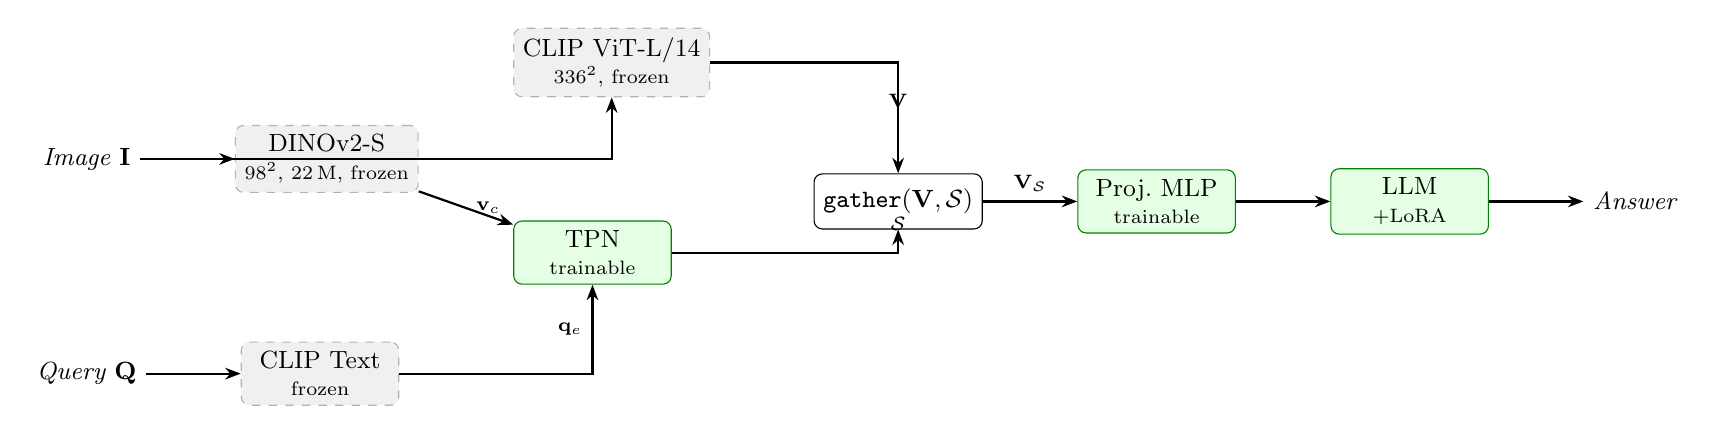
\begin{tikzpicture}[
    node distance=0.6cm and 1.2cm,
    block/.style={rectangle, draw, rounded corners=3pt,
                  minimum height=0.7cm, minimum width=2.0cm,
                  font=\small, align=center, fill=white},
    frozen/.style={block, fill=gray!12, draw=gray!60, dashed},
    trainable/.style={block, fill=green!10, draw=green!50!black},
    data/.style={font=\small\itshape, align=center},
    arr/.style={-{Stealth[scale=0.85]}, thick},
]
  % Input
  \node[data] (img) {Image $\mI$};
  \node[data, below=2.2cm of img] (query) {Query $\mQ$};
  % Encoders
  \node[frozen, right=of img]   (dino) {DINOv2-S\\[-1pt]{\scriptsize $98^2$, 22\,M, frozen}};
  \node[frozen, right=of query] (clip) {CLIP Text\\[-1pt]{\scriptsize frozen}};
  \node[frozen, above right=0.35cm and 1.2cm of dino] (vit)
    {CLIP ViT-L/14\\[-1pt]{\scriptsize $336^2$, frozen}};
  % TPN
  \node[trainable, below right=0.35cm and 1.2cm of dino] (tpn)
    {TPN\\[-1pt]{\scriptsize trainable}};
  % Gather
  \node[block, right=1.8cm of tpn, yshift=0.65cm] (gather)
    {\texttt{gather}$(\mV, \mathcal{S})$};
  % Downstream
  \node[trainable, right=of gather] (mlp) {Proj.~MLP\\[-1pt]{\scriptsize trainable}};
  \node[trainable, right=of mlp]  (llm) {LLM\\[-1pt]{\scriptsize +LoRA}};
  \node[data, right=of llm] (ans) {Answer};
  % Arrows
  \draw[arr] (img)   -- (dino);
  \draw[arr] (img)   -| (vit);
  \draw[arr] (query) -- (clip);
  \draw[arr] (dino)  -- (tpn) node[midway,right,font=\scriptsize]{$\vc$};
  \draw[arr] (clip)  -| (tpn) node[near end,left,font=\scriptsize]{$\qe$};
  \draw[arr] (tpn)   -| (gather) node[near end,above,font=\scriptsize]{$\mathcal{S}$};
  \draw[arr] (vit)   -| (gather) node[near end,above,font=\scriptsize]{$\mV$};
  \draw[arr] (gather)  -- (mlp) node[midway,above,font=\scriptsize]{$\mV_\mathcal{S}$};
  \draw[arr] (mlp)   -- (llm);
  \draw[arr] (llm)   -- (ans);
\end{tikzpicture}
\caption{
  \textbf{TC-ViTok system architecture.}
  Gray dashed boxes: frozen pretrained components.
  Green boxes: trainable components (TPN, projection MLP, LoRA adapters).
  The TPN produces a token index set $\mathcal{S}$ conditioned on the
  query embedding $\qe$ and coarse visual features $\vc$.
  Selected tokens are extracted from the full ViT-L output $\mV$ via
  \texttt{gather}, producing a compact sequence
  $\mV_\mathcal{S} \in \R^{k \times d_v}$ that enters the LLM.
  The LLM prefill sequence length is $k{+}L$ rather than $N{+}L$.
}
\label{fig:architecture}
\end{figure}

TC-ViTok consists of five components (\cref{fig:architecture}):
(1)~a coarse visual encoder,
(2)~a text encoder,
(3)~the Tokenization Policy Network (TPN),
(4)~a full visual encoder with gather-based token extraction, and
(5)~the VLM backbone with LoRA adapters.
Components (1), (2), and (4) are frozen; only (3) and (5) are trained.

\subsection{Coarse Visual Encoder}
\label{subsec:coarse_enc}

The TPN needs a spatial feature map of the image to score spatial positions.
Using the full CLIP ViT-L/14 (304\,M parameters) for this purpose would
negate the efficiency goal.
We instead use DINOv2-Small~\citep{oquab2023dinov2} (22\,M parameters, all
frozen) at a reduced resolution of $98{\times}98$ pixels with patch size~14,
yielding $M = 7 \times 7 = 49$ spatial tokens with embedding dimension
$d_c{=}384$.

\paragraph{Why DINOv2 rather than CLIP for coarse features?}
DINOv2 is trained with a self-supervised local-feature objective, producing
spatial-token representations that correspond faithfully to image regions.
CLIP is trained to collapse spatial structure into a global embedding for
image--text matching; its intermediate spatial tokens are less geometrically
interpretable~\citep{oquab2023dinov2} and thus provide weaker spatial
guidance.

\subsection{Text Encoder}
\label{subsec:text_enc}

We use the frozen CLIP ViT-B/32 text encoder~\citep{radford2021learning} to
produce $\qe \in \R^{512}$, the \texttt{[EOS]} token embedding of the
query.
CLIP training concentrates the global query semantics in the \texttt{[EOS]}
position; mean-pooling would dilute this with padding tokens.

\begin{notebox}[title={Cross-space alignment}]
The query embedding $\qe$ (CLIP text space, $\R^{512}$) and the coarse visual
features $\vc$ (DINOv2 space, $\R^{384}$) reside in different embedding
spaces.
The learned projection matrices $\mathbf{W}^Q$ and $\mathbf{W}^K$ inside the
TPN map both into a shared $d_{\mathrm{model}}$-dimensional space.
This alignment is \emph{learned}, not assumed.
\end{notebox}

\subsection{Tokenization Policy Network (TPN)}
\label{subsec:tpn}

The TPN is a lightweight module (all trainable) that maps
$(\qe, \vc) \mapsto \vs_N \in \R^N$, producing a relevance score for each
of the $N$ full-resolution visual tokens.
It consists of three stages: cross-attention, scoring, and upsampling.

\subsubsection{Stage 1: Cross-Attention}

The query embedding $\qe$ (a single vector) attends to the $M{=}49$ coarse
spatial tokens:

\begin{definitionbox}[title={TPN Cross-Attention}]
Let $H$ denote the number of attention heads and $d_k = d_{\mathrm{model}}/H$.
\begin{align}
  \mathbf{Q}_{\mathrm{attn}} &= \qe\, \mathbf{W}^Q \in \R^{1 \times d_{\mathrm{model}}},
    &\quad \mathbf{W}^Q &\in \R^{d_q \times d_{\mathrm{model}}} \label{eq:q_proj} \\
  \mathbf{K}_{\mathrm{attn}} &= \vc\, \mathbf{W}^K \in \R^{M \times d_{\mathrm{model}}},
    &\quad \mathbf{W}^K &\in \R^{d_c \times d_{\mathrm{model}}} \label{eq:k_proj} \\
  \mathbf{V}_{\mathrm{attn}} &= \vc\, \mathbf{W}^V \in \R^{M \times d_{\mathrm{model}}},
    &\quad \mathbf{W}^V &\in \R^{d_c \times d_{\mathrm{model}}} \label{eq:v_proj}
\end{align}
For each head $h \in \{1,\ldots,H\}$:
\begin{align}
  \boldsymbol{\alpha}^{(h)}
    &= \Softmax\!\Bigl(
      \frac{\mathbf{Q}_{\mathrm{attn}}^{(h)}\,
            {\mathbf{K}_{\mathrm{attn}}^{(h)}}^\top}
           {\sqrt{d_k}}
    \Bigr) \in \R^{1 \times M}, \label{eq:attn_weights} \\[3pt]
  \mathbf{a}^{(h)}
    &= \boldsymbol{\alpha}^{(h)}\, \mathbf{V}_{\mathrm{attn}}^{(h)}
    \in \R^{1 \times d_k}. \label{eq:attn_out}
\end{align}
Multi-head outputs are concatenated and projected:
\begin{equation}
  \mathbf{a} = \Concat\!\bigl(\mathbf{a}^{(1)}, \ldots,
    \mathbf{a}^{(H)}\bigr)\, \mathbf{W}^O
    \in \R^{1 \times d_{\mathrm{model}}},
  \qquad \mathbf{W}^O \in \R^{d_{\mathrm{model}} \times d_{\mathrm{model}}}.
  \label{eq:multihead}
\end{equation}
\end{definitionbox}

\paragraph{Attention weight aggregation.}
\begin{equation}
  \bar{\boldsymbol{\alpha}} =
    \frac{1}{H} \sum_{h=1}^{H} \boldsymbol{\alpha}^{(h)}
    \;\in \R^{1 \times M}.
  \label{eq:alpha_avg}
\end{equation}

\subsubsection{Stage 2: Spatial Scoring}

\begin{align}
  \mathbf{h} &= \mathrm{GELU}\!\bigl(
    \mathbf{W}_1 \,
    [\,\underbrace{\mathbf{a}^{\flat}}_{\in\,\R^{d_{\mathrm{model}}}};\;
     \underbrace{\bar{\boldsymbol{\alpha}}^{\flat}}_{\in\,\R^{M}}\,]
    + \mathbf{b}_1
  \bigr) \in \R^{d_h},
  \label{eq:mlp_hidden} \\
  \vs_M &= \mathbf{W}_2\, \mathbf{h} + \mathbf{b}_2 \in \R^{M}.
  \label{eq:score_coarse}
\end{align}

\subsubsection{Stage 3: Spatial Upsampling}

\begin{equation}
  \vs_N = \flatten\!\Bigl(
    \Upsample\!\bigl(
      \reshape(\vs_M,\; 7, 7),\;
      (24, 24)
    \bigr)
  \Bigr) \;\in\; \R^{N}.
  \label{eq:upsample}
\end{equation}

\subsubsection{Token Selection}

At inference, the top-$k$ indices determine the selected tokens:
\begin{equation}
  \mathcal{S} = \TopK(\vs_N,\, k)
    = \{i : s_{N,i} \text{ is among the $k$ largest values}\}.
  \label{eq:topk}
\end{equation}
During training, this non-differentiable operation is replaced by the
Gumbel-Sigmoid STE (\cref{sec:gumbel}).

\subsection{Gather-Based Token Extraction and Downstream Processing}
\label{subsec:gather}

The full visual encoder (CLIP ViT-L/14, frozen) processes the original
$336{\times}336$ image to produce $\mV \in \R^{576 \times 1024}$.
The selected token set $\mathcal{S}$ is used to extract a compact visual
sequence via index-gather:

\begin{equation}
  \mV_{\mathcal{S}} = \mV[\mathcal{S},\, :] \;\in\; \R^{k \times d_v},
  \label{eq:gather}
\end{equation}

where $\mV[\mathcal{S}, :]$ denotes selecting the rows of $\mV$ indexed by
$\mathcal{S}$.
In PyTorch this is implemented as:
\begin{equation}
  \texttt{idx} = \vs_N.\texttt{topk}(k).\texttt{indices},
  \qquad
  \mV_\mathcal{S} = \texttt{torch.gather}(\mV,\; \texttt{dim}{=}1,\;
    \texttt{idx.unsqueeze(-1).expand(-1,-1,}d_v\texttt{)}).
\end{equation}

The resulting $\mV_\mathcal{S} \in \R^{k \times d_v}$ (not $N \times d_v$)
passes through LLaVA-1.5's two-layer MLP projector
($\R^{1024} \to \R^{4096}$), yielding $k$ projected visual tokens.
These are concatenated with text-token embeddings to form a sequence of
length $k{+}L$, which is processed by the LLM backbone with
LoRA~\citep{hu2022lora} adapters on $\{Q,K,V,O\}$ projections.

\begin{remark}[Locus of compute savings]
  \label{rem:savings}
  The full ViT-L processes all $N{=}576$ patches before gather; no savings
  accrue in the vision encoder.
  All compute savings are realized in the LLM: the gather operation reduces
  the prefill sequence from $N{+}L$ to $k{+}L$ tokens.
  At $k{=}144$, this cuts the dominant $\mathcal{O}(N(N{+}L))$ LLM prefill
  cost by approximately $75\%$.
  An alternative zero-masking approach (multiplying $\mV$ by a binary mask
  and retaining all $N$ rows) would save only KV-cache memory, not FLOPs,
  and is therefore not adopted.
  True pre-ViT savings---where unselected patches skip ViT self-attention
  entirely---would require a sparse-attention ViT and are left to future work.
\end{remark}

\paragraph{Computational overhead of the TPN pipeline.}
The TPN adds three inference-time costs that partially offset the LLM savings:
(i)~DINOv2-S forward pass (22\,M params, $\sim$3\,ms on A100),
(ii)~CLIP text encoding ($\sim$2\,ms), and
(iii)~TPN forward pass ($\sim$0.5\,ms).
Total overhead is $\sim$5.5\,ms, compared to LLM prefill savings of
$\sim$40\,ms at $k{=}144$ (batch size~1, Vicuna-7B, using gather).
Net wall-clock savings are thus $\sim$34\,ms per sample.

% ════════════════════════════════════════════════════════════════════════════
\section{Differentiable Token Selection}
\label{sec:gumbel}
% ════════════════════════════════════════════════════════════════════════════

\subsection{The Non-Differentiability Problem}

The $\TopK$ operation is a discrete map with zero gradients almost everywhere,
blocking gradient flow from $\mathcal{L}_{\mathrm{VQA}}$ through the
selection to the TPN parameters~$\theta$.
We require a differentiable surrogate for training.

\subsection{Gumbel-Sigmoid for Independent Binary Selection}

Because we select a \emph{subset} of tokens (not a single token), we use the
Gumbel-Sigmoid rather than the Gumbel-Softmax.
Gumbel-Sigmoid treats each token's inclusion as an independent binary
decision.

\begin{definitionbox}[title={Gumbel-Sigmoid Soft Mask}]
Let $g_i = -\log(-\log(u_i))$ with $u_i \sim \mathrm{Uniform}(0,1)$
(clamped: $u_i \in [\epsilon, 1{-}\epsilon]$, $\epsilon{=}10^{-8}$).
The temperature-controlled soft mask is:
\begin{equation}
  \tilde{m}_i(\tau)
    = \sigma\!\!\left(\frac{s_{N,i} + g_i}{\tau}\right),
  \label{eq:gumbel_sigmoid}
\end{equation}
where $\sigma$ is the logistic sigmoid.
\end{definitionbox}

\paragraph{Temperature annealing.}
\begin{equation}
  \tau(t) = \tau_{\max} - (\tau_{\max} - \tau_{\min})
    \cdot \frac{t}{T},
  \label{eq:tau_anneal}
\end{equation}
with $\tau_{\max}{=}1.0$, $\tau_{\min}{=}0.1$, and $T$ the total training
steps.

\subsection{Straight-Through Estimator (STE)}

During training, the STE uses the hard top-$k$ indices in the forward pass
but routes gradients through the differentiable Gumbel-Sigmoid:

\begin{definitionbox}[title={Straight-Through Estimator for Top-$k$ Selection}]
\begin{align}
  \vm_{\mathrm{hard}}
    &= \mathbf{1}\bigl[\vs_N \geq \tau_k(\vs_N)\bigr],
    && \text{(hard mask, forward pass)}
    \label{eq:hard_mask} \\[3pt]
  \tilde{\vm}(\tau)
    &= \sigma\!\bigl((\vs_N + \mathbf{g})\,/\,\tau\bigr),
    && \text{(soft mask, backward-pass gradients)}
    \label{eq:soft_mask} \\[3pt]
  \vm_{\mathrm{STE}}
    &= \vm_{\mathrm{hard}} - \sg{\tilde{\vm}(\tau)} + \tilde{\vm}(\tau).
    \label{eq:ste}
\end{align}
\end{definitionbox}

During training, gather is applied using indices derived from
$\vm_{\mathrm{STE}}$ (i.e., positions where $\vm_{\mathrm{STE}} = 1$),
so gradients flow through $\tilde{\vm}$ to the TPN parameters $\theta$.

% ════════════════════════════════════════════════════════════════════════════
\section{Training}
\label{sec:training}
% ════════════════════════════════════════════════════════════════════════════

\subsection{Complete Training Loss}

\begin{equation}
  \mathcal{L}(t) = \mathcal{L}_{\mathrm{VQA}}
    + \lambda(t)\, \frac{\lVert \vs_N \rVert_1}{N}
    + \mu\, \mathcal{L}_{\mathrm{ent}},
  \label{eq:total_loss}
\end{equation}
where $\lambda(t) = \lambda_{\max} \cdot \min(1, t/T_{\mathrm{warmup}})$
and $\mathcal{L}_{\mathrm{ent}}$ is the spatial-entropy regularizer
(\cref{subsec:spatial_collapse}).

\subsection{Phased Training Protocol}

\paragraph{Phase~0: TPN warm-up (1 epoch).}
Only TPN parameters $\theta$ are trained.
Loss: $\mathcal{L}_{\mathrm{VQA}}$ only.
Temperature: $\tau{=}1.0$.

\paragraph{Phase~1: Joint fine-tuning (3 epochs).}
Trainable: TPN, LoRA adapters (rank~32, $\alpha{=}64$), projection MLP.
Loss: $\mathcal{L}(t)$ with $\lambda$ and $\tau$ annealing.
Optimizer: AdamW with per-group learning rates
($\eta_{\mathrm{TPN}}{=}10^{-3}$,
$\eta_{\mathrm{LoRA}}{=}2{\times}10^{-4}$,
$\eta_{\mathrm{MLP}}{=}5{\times}10^{-4}$),
weight decay $0.01$, gradient clipping $\lVert\nabla_\theta\rVert_2 \leq 1$.

\begin{algorithm}[t]
\caption{TC-ViTok Training}
\label{alg:training}
\begin{algorithmic}[1]
\Require Dataset $\mathcal{D}$, budget $k$, $\lambda_{\max}$, $\mu$,
  $\tau_{\max}$, $\tau_{\min}$, total steps $T$
\State Initialize TPN $\theta$; load frozen encoders; apply LoRA to LLM
\Statex \hrulefill\ \textbf{Phase~0: TPN warm-up}\ \hrulefill
\For{1 epoch over $\mathcal{D}$}
  \State $\vc \gets \mathrm{DINOv2\text{-}S}(\mathrm{resize}(\mI, 98^2))$
  \State $\qe \gets \mathrm{CLIPText}(\mQ)$
  \State $\vs_N \gets \mathrm{TPN}_\theta(\vc, \qe)$;\;
    $\vm_{\mathrm{STE}} \gets \mathrm{GumbelSTE}(\vs_N, k, \tau{=}1.0)$
  \State $\mV \gets \mathrm{ViT\text{-}L}(\mI)$
  \State $\mathcal{S} \gets \mathrm{indices}(\vm_{\mathrm{STE}})$;\;
    $\mV_\mathcal{S} \gets \mathrm{gather}(\mV, \mathcal{S})$
    \Comment{$(B,k,d_v)$}
  \State $\hat{A} \gets f_{\mathrm{LLM}}(\mQ,\, \mV_\mathcal{S})$
    \Comment{LLM frozen; sees $k{+}L$ tokens}
  \State $\theta \gets \theta - \eta_{\mathrm{TPN}}\,
    \nabla_\theta \mathcal{L}_{\mathrm{VQA}}(\hat{A}, A)$
\EndFor
\Statex \hrulefill\ \textbf{Phase~1: Joint fine-tuning}\ \hrulefill
\For{$t = 1, \ldots, T$}
  \State $\tau \gets \tau(t)$;\; $\lambda \gets \lambda(t)$
  \State Compute $\vs_N$, $\vm_{\mathrm{STE}}$, $\mathcal{S}$,
    $\mV_\mathcal{S}$ as above
  \State $\hat{A} \gets f_{\mathrm{LLM}}^{\mathrm{LoRA}}(\mQ,\, \mV_\mathcal{S})$
  \State $\mathcal{L} \gets \mathcal{L}_{\mathrm{VQA}}
    + \lambda\,\lVert\vs_N\rVert_1/N
    + \mu\,\mathcal{L}_{\mathrm{ent}}$
  \State Update $\theta$, LoRA, MLP via AdamW
\EndFor
\end{algorithmic}
\end{algorithm}

\subsection{Failure Modes and Mitigations}
\label{subsec:failures}

\subsubsection{Spatial Collapse (Center Bias)}
\label{subsec:spatial_collapse}

\begin{warnbox}[title={Failure Mode 1: Spatial Collapse}]
\textbf{Symptom:} The TPN selects center-image tokens regardless of query.
\textbf{Mitigation:} Spatial-entropy regularizer.
\end{warnbox}

\paragraph{Mitigation: spatial-entropy regularizer.}
\begin{equation}
  \hat{p}_i = \frac{\bar{m}_i}{\sum_{j=1}^N \bar{m}_j + \epsilon},
  \qquad
  \mathcal{L}_{\mathrm{ent}}
    = -\sum_{i=1}^{N} \hat{p}_i \log(\hat{p}_i + \epsilon),
  \label{eq:entropy_reg}
\end{equation}
maximized with coefficient $|\mu|{=}0.01$.

\subsubsection{Query Ignoring}

\begin{warnbox}[title={Failure Mode 2: Query Ignoring}]
\textbf{Symptom:}
$\IoU(\mathcal{S}(\qe^{(1)},\vc),\; \mathcal{S}(\qe^{(2)},\vc)) \approx 1$
for different queries on the same image.
\textbf{Mitigation:} Query-diversity loss (\cref{eq:div_loss}).
\end{warnbox}

\begin{equation}
  \mathcal{L}_{\mathrm{div}} = \sum_{b=1}^{B}
    \max\!\bigl(0,\;\simop(\vm^{(b)}_1,\vm^{(b)}_2) - \gamma\bigr)
    \cdot
    \bigl(1 - \simop(\qe^{(b)}_1, \qe^{(b)}_2)\bigr).
  \label{eq:div_loss}
\end{equation}

\subsubsection{Degenerate Fixed Mask}

\begin{warnbox}[title={Failure Mode 3: Degenerate Fixed Mask}]
\textbf{Symptom:} Same $k$ tokens selected for every input.
\textbf{Fix:} Reduce $\lambda_{\max}$ by $10\times$; increase
$T_{\mathrm{warmup}}$.
\end{warnbox}

% ════════════════════════════════════════════════════════════════════════════
\section{Experimental Design}
\label{sec:experiments}
% ════════════════════════════════════════════════════════════════════════════

\subsection{Setup}

\paragraph{Backbone.}
LLaVA-1.5-7B~\citep{liu2024llava} (CLIP ViT-L/14, Vicuna-7B).
Token budget: $k{=}144$ ($4\times$ compression) unless otherwise stated.

\paragraph{Datasets.}
VQAv2~\citep{goyal2017vqa}, GQA~\citep{hudson2019gqa}, TextVQA, and
POPE~\citep{pope}.

\paragraph{Metrics.}
VQA-Score, GQA exact-match accuracy (balanced test), POPE F1, and
end-to-end inference latency at batch size~1 on A100 using gather.

\subsection{Baselines}

\begin{table}[h]
\centering
\caption{Baselines. All use LLaVA-1.5-7B at $k{=}144$ tokens except the
full model ($N{=}576$).}
\label{tab:baselines}
\renewcommand{\arraystretch}{1.15}
\small
\begin{tabular}{@{}lccp{5.5cm}@{}}
  \toprule
  Condition & Query-aware & Tokens & Description \\
  \midrule
  LLaVA-1.5 (full)   & N/A & 576 & Upper bound (no compression) \\
  Random drop         & No  & 144 & Uniformly random gather \\
  ToMe~\citep{bolya2022token} & No & 144 & Bipartite soft matching \\
  Image-only TPN (A3) & No  & 144 & TPN without query input \\
  \textbf{TC-ViTok}   & \textbf{Yes} & \textbf{144} & Full method \\
  \bottomrule
\end{tabular}
\end{table}

All compression conditions use gather (sequence length $k{+}L$) for a
fair latency comparison.

\subsection{Spatial Specificity Evaluation Protocol}
\label{subsec:spatial_protocol}

Questions are classified as \emph{spatial} or \emph{global} using:
\begin{enumerate}[leftmargin=1.5em, itemsep=1pt]
  \item (GQA only) \texttt{relation.spatial = True}.
  \item Answer is a spatial direction.
  \item Question contains spatial keywords.
\end{enumerate}

\subsection{Ablation Studies}

\begin{table}[h]
\centering
\caption{Ablation matrix.}
\label{tab:ablations}
\renewcommand{\arraystretch}{1.15}
\small
\begin{tabular}{@{}llp{5.5cm}@{}}
  \toprule
  ID & Variation & Tests \\
  \midrule
  A1 & Full TC-ViTok       & Full system \\
  A2 & Random drop          & Absolute lower bound \\
  A3 & Image-only TPN       & Value of query-conditioning \\
  A4 & $k \in \{72,144,216,288\}$ & Pareto frontier \\
  A5 & Spatial vs.\ global split & \Cref{hyp:main} \\
  \midrule
  B1 & Skip Phase~0         & Cold-start importance \\
  B2 & Fixed $\tau{=}1.0$   & Annealing importance \\
  B3 & DINOv2-S vs.\ CLIP-B coarse enc. & Encoder suitability \\
  \bottomrule
\end{tabular}
\end{table}

\subsection{Hypotheses}

\begin{hypothesis}[Query-Conditioning Selectivity]
  \label{hyp:main}
  \begin{align}
    \mathrm{Acc}(\text{A1},\,\text{spatial})
      &> \mathrm{Acc}(\text{A3},\,\text{spatial}), \\
    |\mathrm{Acc}(\text{A1},\,\text{global})
      - \mathrm{Acc}(\text{A3},\,\text{global})|
      &\approx 0.
  \end{align}
\end{hypothesis}

\begin{hypothesis}[Pareto Dominance]
  \label{hyp:pareto}
  The accuracy-vs-tokens Pareto curve of TC-ViTok lies at or above those
  of all query-agnostic baselines for $k \in \{72, 144, 216, 288\}$.
\end{hypothesis}

\subsection{Projected Quantitative Outcomes}

\begin{table}[h]
\centering
\caption{
  \textbf{Projected} results (not yet measured).
}
\label{tab:projected}
\renewcommand{\arraystretch}{1.2}
\small
\begin{tabular}{@{}lccccr@{}}
  \toprule
  Method & VQAv2 & GQA & GQA-spat. & POPE-F1 & Tokens \\
  \midrule
  LLaVA-1.5 (full)    & 79.1 & 63.3 & 62.1 & 85.9 & 576 \\
  Random drop          & $\sim$72 & $\sim$57 & $\sim$53 & $\sim$81 & 144 \\
  ToMe                 & $\sim$74 & $\sim$59 & $\sim$55 & $\sim$83 & 144 \\
  Image-only TPN (A3)  & $\sim$75 & $\sim$60 & $\sim$56 & $\sim$83 & 144 \\
  \textbf{TC-ViTok}    & $\mathbf{\sim\!76}$ & $\mathbf{\sim\!61}$
    & $\mathbf{\sim\!59}$ & $\mathbf{\sim\!84}$ & \textbf{144} \\
  \bottomrule
\end{tabular}
\end{table}

% ════════════════════════════════════════════════════════════════════════════
\section{Discussion}
\label{sec:discussion}
% ════════════════════════════════════════════════════════════════════════════

\subsection{Novelty and Positioning}

\paragraph{Conceptual novelty.}
No prior work frames visual tokenization in VLMs as a query-conditioned
policy.
Existing compression methods are query-agnostic; conditional feature
extraction in BLIP-2 uses learned queries rather than the user's
natural-language question.

\paragraph{Architectural novelty.}
The TPN cross-attention module---bridging a CLIP text embedding and DINOv2
spatial features to produce a sparse selection for a separate full-resolution
encoder, realized via gather before LLM injection---has no direct precedent.

\paragraph{Evaluation novelty.}
The spatial specificity stratification protocol, leveraging GQA's semantic
annotations, is (to our knowledge) not previously used for evaluating VLM
efficiency methods.

\subsection{Limitations}

\begin{itemize}[leftmargin=1.5em, itemsep=2pt]
  \item \textbf{Post-ViT gather only.}
    The full ViT-L processes all $N$ tokens before gather.
    True pre-ViT savings require a sparse-attention ViT.
  \item \textbf{Coarse spatial resolution.}
    The TPN operates on a $7{\times}7$ grid (upsampled to $24{\times}24$).
  \item \textbf{STE bias.}
    Reduced but not eliminated by temperature annealing.
  \item \textbf{No measured results.}
    The experimental section currently reports projected values.
\end{itemize}

% ════════════════════════════════════════════════════════════════════════════
\section{Conclusion}
\label{sec:conclusion}
% ════════════════════════════════════════════════════════════════════════════

We introduced TC-ViTok, a framework for query-conditioned visual
tokenization in vision-language models.
The Tokenization Policy Network produces a sparse token selection conditioned
on the user's language query; selected tokens are extracted via index-gather
before LLM injection, reducing LLM prefill sequence length from $N{+}L$ to
$k{+}L$ and cutting prefill FLOPs by up to $75\%$.
The framework makes a precise, testable prediction---that query-conditioning
helps selectively on spatially-grounded questions---and provides the
evaluation protocol to test it.

% ════════════════════════════════════════════════════════════════════════════
\appendix
\section{Implementation Details}
\label{app:implementation}
% ════════════════════════════════════════════════════════════════════════════

\subsection{TPN Parameter Count}

With $d_q{=}512$, $d_c{=}384$, $d_{\mathrm{model}}{=}384$, $H{=}4$,
$d_h{=}512$, and $M{=}49$:

\begin{center}
\small
\renewcommand{\arraystretch}{1.15}
\begin{tabular}{@{}lr@{}}
  \toprule
  Component & Parameters \\
  \midrule
  $\mathbf{W}^Q$ ($d_q \times d_{\mathrm{model}}$) & 196\,608 \\
  $\mathbf{W}^K$ ($d_c \times d_{\mathrm{model}}$) & 147\,456 \\
  $\mathbf{W}^V$ ($d_c \times d_{\mathrm{model}}$) & 147\,456 \\
  $\mathbf{W}^O$ ($d_{\mathrm{model}} \times d_{\mathrm{model}}$) & 147\,456 \\
  LayerNorms ($\times 2$) & 1\,536 \\
  Score MLP: $\mathbf{W}_1$ & 221\,696 \\
  Score MLP: $\mathbf{W}_2$ + biases & 25\,137 \\
  \midrule
  \textbf{Total} & \textbf{$\approx$887\,K} \\
  \bottomrule
\end{tabular}
\end{center}

\subsection{Gumbel-Sigmoid STE Implementation}

\begin{lstlisting}[caption={Gumbel-Sigmoid STE for top-$k$ selection
  (PyTorch).}]
import torch

def gumbel_sigmoid_ste(scores, k, tau):
    """
    Args:
        scores: (B, N) raw spatial scores from TPN
        k:      number of tokens to select
        tau:    Gumbel temperature (annealed during training)
    Returns:
        mask: (B, N) with hard values in fwd, soft grads in bwd
    """
    eps = 1e-8
    u = torch.rand_like(scores).clamp(eps, 1 - eps)
    g = -torch.log(-torch.log(u))               # Gumbel(0,1)
    m_soft = torch.sigmoid((scores + g) / tau)   # soft mask

    topk_idx = scores.topk(k, dim=-1).indices    # (B, k)
    m_hard = torch.zeros_like(scores)
    m_hard.scatter_(-1, topk_idx, 1.0)

    # STE: fwd = m_hard, bwd = grad through m_soft
    return m_hard - m_soft.detach() + m_soft
\end{lstlisting}

\subsection{TPN Forward Pass and Gather-Based Extraction}

\begin{lstlisting}[caption={TPN module with gather-based token extraction.}]
import torch
import torch.nn as nn
import torch.nn.functional as F

class TPN(nn.Module):
    def __init__(self, d_q=512, d_c=384, d_model=384,
                 n_heads=4, d_h=512, M=49, N=576):
        super().__init__()
        self.q_proj = nn.Linear(d_q, d_model, bias=False)
        self.k_proj = nn.Linear(d_c, d_model, bias=False)
        self.v_proj = nn.Linear(d_c, d_model, bias=False)
        self.o_proj = nn.Linear(d_model, d_model, bias=False)
        self.n_heads = n_heads
        self.d_k = d_model // n_heads
        self.norm1 = nn.LayerNorm(d_model)
        self.norm2 = nn.LayerNorm(d_model + M)
        self.score_mlp = nn.Sequential(
            nn.Linear(d_model + M, d_h),
            nn.GELU(),
            nn.Linear(d_h, M),
        )
        self.sqrt_M = int(M ** 0.5)
        self.sqrt_N = int(N ** 0.5)

    def forward(self, v_c, q_e, k, tau, training=True):
        B = v_c.size(0)
        # Cross-attention
        Q = self.q_proj(q_e).unsqueeze(1)
        K = self.k_proj(v_c)
        V = self.v_proj(v_c)
        Q = Q.view(B, 1, self.n_heads, self.d_k).transpose(1, 2)
        K = K.view(B, -1, self.n_heads, self.d_k).transpose(1, 2)
        V = V.view(B, -1, self.n_heads, self.d_k).transpose(1, 2)
        alpha = (Q @ K.transpose(-2, -1)) / (self.d_k ** 0.5)
        alpha = alpha.softmax(dim=-1)
        ctx = alpha @ V
        ctx = ctx.transpose(1, 2).reshape(B, 1, -1)
        ctx = self.o_proj(ctx).squeeze(1)
        ctx = self.norm1(ctx)
        alpha_avg = alpha.mean(dim=1).squeeze(-2)
        combined = torch.cat([ctx, alpha_avg], dim=-1)
        s_M = self.score_mlp(self.norm2(combined))
        s = s_M.view(B, 1, self.sqrt_M, self.sqrt_M)
        s = F.interpolate(s, (self.sqrt_N, self.sqrt_N),
                          mode='bilinear', align_corners=False)
        s_N = s.view(B, -1)                          # (B, N)

        if training:
            mask_ste = gumbel_sigmoid_ste(s_N, k, tau)
            # Derive gather indices from STE mask
            idx = mask_ste.topk(k, dim=-1).indices   # (B, k)
        else:
            idx = s_N.topk(k, dim=-1).indices        # (B, k)

        return idx, s_N   # return indices, not mask


def gather_tokens(V, idx):
    """
    Extract k visual tokens from V using top-k indices.
    Args:
        V:   (B, N, d_v)  full ViT-L visual tokens
        idx: (B, k)       selected token indices
    Returns:
        V_selected: (B, k, d_v)  compact visual sequence
    """
    d_v = V.shape[-1]
    idx_exp = idx.unsqueeze(-1).expand(-1, -1, d_v)  # (B, k, d_v)
    return torch.gather(V, dim=1, idx_exp)            # (B, k, d_v)
\end{lstlisting}

\begin{lstlisting}[caption={TCViTok forward pass using gather.}]
class TCViTok(nn.Module):
    def forward(self, pixel_values, input_ids, labels,
                v_c, q_e, tau=1.0, training=True):
        # Step 1: Full visual tokens (frozen ViT-L)
        with torch.no_grad():
            V = self.vit(pixel_values).last_hidden_state[:, 1:, :]
            # V: (B, 576, 1024)

        # Step 2: TPN produces top-k indices
        idx, s_N = self.tpn(v_c, q_e, self.k, tau, training)
        # idx: (B, 144)

        # Step 3: Gather -- LLM receives k tokens, not N
        V_selected = gather_tokens(V, idx)
        # V_selected: (B, 144, 1024)  <-- sequence shortened here

        # Step 4: Project and forward
        V_proj = self.projector(V_selected)
        # V_proj: (B, 144, 4096)

        text_embeds = self.llm.model.embed_tokens(input_ids)
        combined = torch.cat([V_proj, text_embeds], dim=1)
        # combined: (B, 144+L, 4096)  <-- real savings here

        outputs = self.llm(inputs_embeds=combined, labels=labels)
        return outputs.loss, s_N, idx
\end{lstlisting}

\begin{lstlisting}[caption={Inference with gather.}]
@torch.no_grad()
def inference(model, pixel_values, input_ids, v_c, q_e, k=144):
    model.eval()
    V = model.vit(pixel_values).last_hidden_state[:, 1:, :]
    idx, s_N = model.tpn(v_c, q_e, k, tau=0.1, training=False)
    V_selected = gather_tokens(V, idx)   # (B, k, 1024)
    V_proj = model.projector(V_selected)
    # ... autoregressive generation with V_proj prefix ...
    return answer, idx


def visualize_mask(image, selected_idx, question, k=144, N=576):
    """Accepts gather indices; converts to 2D heatmap for display."""
    import torch, matplotlib.pyplot as plt
    mask = torch.zeros(N)
    mask[selected_idx.cpu()] = 1.0
    mask_2d = mask.reshape(24, 24).numpy()

    fig, axes = plt.subplots(1, 3, figsize=(15, 5))
    axes[0].imshow(image); axes[0].set_title("Original")
    axes[1].imshow(mask_2d, cmap='hot', interpolation='nearest')
    axes[1].set_title(f"Selected (k={k})")
    axes[2].imshow(image, alpha=0.5)
    axes[2].imshow(mask_2d, cmap='Greens', alpha=0.4)
    axes[2].set_title(f"Q: {question[:50]}...")
    plt.tight_layout()
    plt.savefig('mask_viz.pdf', dpi=150)
\end{lstlisting}

\subsection{LoRA Configuration}

\begin{lstlisting}[caption={LoRA setup via PEFT.}, numbers=none]
from peft import LoraConfig, get_peft_model, TaskType

config = LoraConfig(
    task_type=TaskType.CAUSAL_LM,
    r=32, lora_alpha=64,
    target_modules=["q_proj", "k_proj", "v_proj", "o_proj"],
    lora_dropout=0.05, bias="none",
)
model.llm = get_peft_model(model.llm, config)
\end{lstlisting}

% ════════════════════════════════════════════════════════════════════════════
\begin{thebibliography}{99}

\bibitem{bai2023qwenvl}
Bai, J., et al.\ (2023). Qwen-VL. \emph{arXiv:2308.12966}.

\bibitem{bengio2013estimating}
Bengio, Y., L\'{e}onard, N., \& Courville, A.\ (2013).
Estimating or propagating gradients through stochastic neurons.
\emph{arXiv:1308.3432}.

\bibitem{bolya2022token}
Bolya, D., et al.\ (2023). Token merging. In \emph{ICLR}.

\bibitem{goyal2017vqa}
Goyal, Y., et al.\ (2017). Making the V in VQA matter. In \emph{CVPR}.

\bibitem{hu2022lora}
Hu, E.~J., et al.\ (2022). LoRA. In \emph{ICLR}.

\bibitem{hudson2019gqa}
Hudson, D.~A., \& Manning, C.~D.\ (2019). GQA. In \emph{CVPR}.

\bibitem{jang2017categorical}
Jang, E., Gu, S., \& Poole, B.\ (2017).
Categorical reparameterization with Gumbel-Softmax. In \emph{ICLR}.

\bibitem{li2023blip2}
Li, J., et al.\ (2023). BLIP-2. In \emph{ICML}.

\bibitem{liang2022evit}
Liang, Y., et al.\ (2022). Not all patches are what you need. In \emph{ICLR}.

\bibitem{liu2024llava}
Liu, H., et al.\ (2023). Visual instruction tuning. In \emph{NeurIPS}.

\bibitem{maddison2017concrete}
Maddison, C.~J., Mnih, A., \& Teh, Y.~W.\ (2017).
The Concrete distribution. In \emph{ICLR}.

\bibitem{meng2022adavit}
Meng, L., et al.\ (2022). AdaViT. In \emph{CVPR}.

\bibitem{oquab2023dinov2}
Oquab, M., et al.\ (2023). DINOv2. \emph{arXiv:2304.07193}.

\bibitem{pope}
Li, Y., et al.\ (2023). Evaluating object hallucination. In \emph{EMNLP}.

\bibitem{radford2021learning}
Radford, A., et al.\ (2021).
Learning transferable visual models. In \emph{ICML}.

\bibitem{rao2021dynamicvit}
Rao, Y., et al.\ (2021). DynamicViT. In \emph{NeurIPS}.

\bibitem{shang2024llava}
Shang, Y., et al.\ (2024). LLaVA-PruMerge. \emph{arXiv:2403.15388}.

\bibitem{shazeer2017moe}
Shazeer, N., et al.\ (2017). Sparsely-gated mixture-of-experts. In \emph{ICLR}.

\bibitem{teerapittayanon2016branchynet}
Teerapittayanon, S., et al.\ (2016). BranchyNet. In \emph{ICPR}.

\end{thebibliography}

\end{document}